\part{Entrega 1}

\begin{center}
    \href{https://github.com/LukasWolff2002/PROYECTO_1_MCOC_ENTREGA_1}{Ver repositorio GitHub.}
\end{center}

\setcounter{section}{0}

\section{Introducción}

\section{Marco Teórico}

\subsection{Ley de Darcy}

La ley de Darcy expone lo siguiente

\begin{equation}
    q = k \cdot i \cdot A
\end{equation}

Lo que es analogo a:

\begin{equation}
    v = k \cdot i
\end{equation}

Donde i es el gradiente hidraulico, dicretizandolo en el espacio, se obtiene lo siguiente:

\begin{equation}
    i = \frac{dh}{dl} = \frac{dh}{dx};\frac{dh}{dy};\frac{dh}{dz}
\end{equation}

Sea lo siguiente:

\begin{figure}[H]
    \centering
    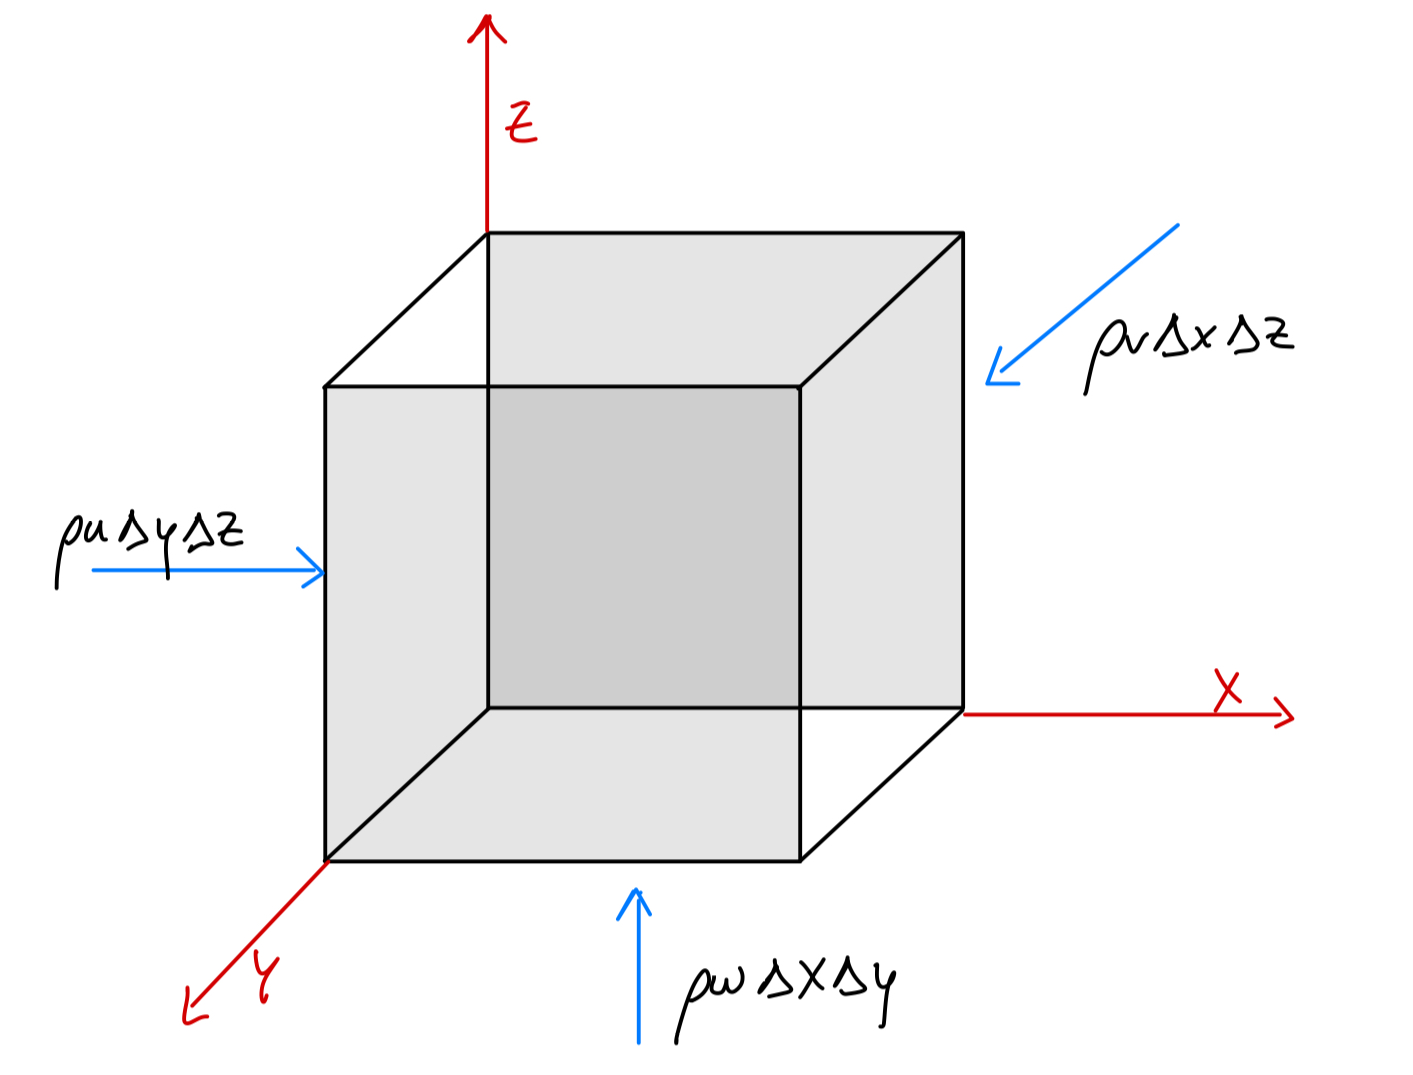
\includegraphics[width=0.5\textwidth]{FOTOS/in.jpg}
    \caption{Ingreso al Sistema}
    \label{fig:ley_darcy}
\end{figure}

La serie de Taylor expone que:

\begin{equation}
    f(x) = f(a) + \frac{df(a) \Delta X}{dx \cdot 1!} + ... + \frac{\Delta X^n}{n!} \cdot \frac{d^n f(a)}{dx^n}
\end{equation}

Por lo tanto, lo que sale del sistema es:

\begin{figure}[H]
    \centering
    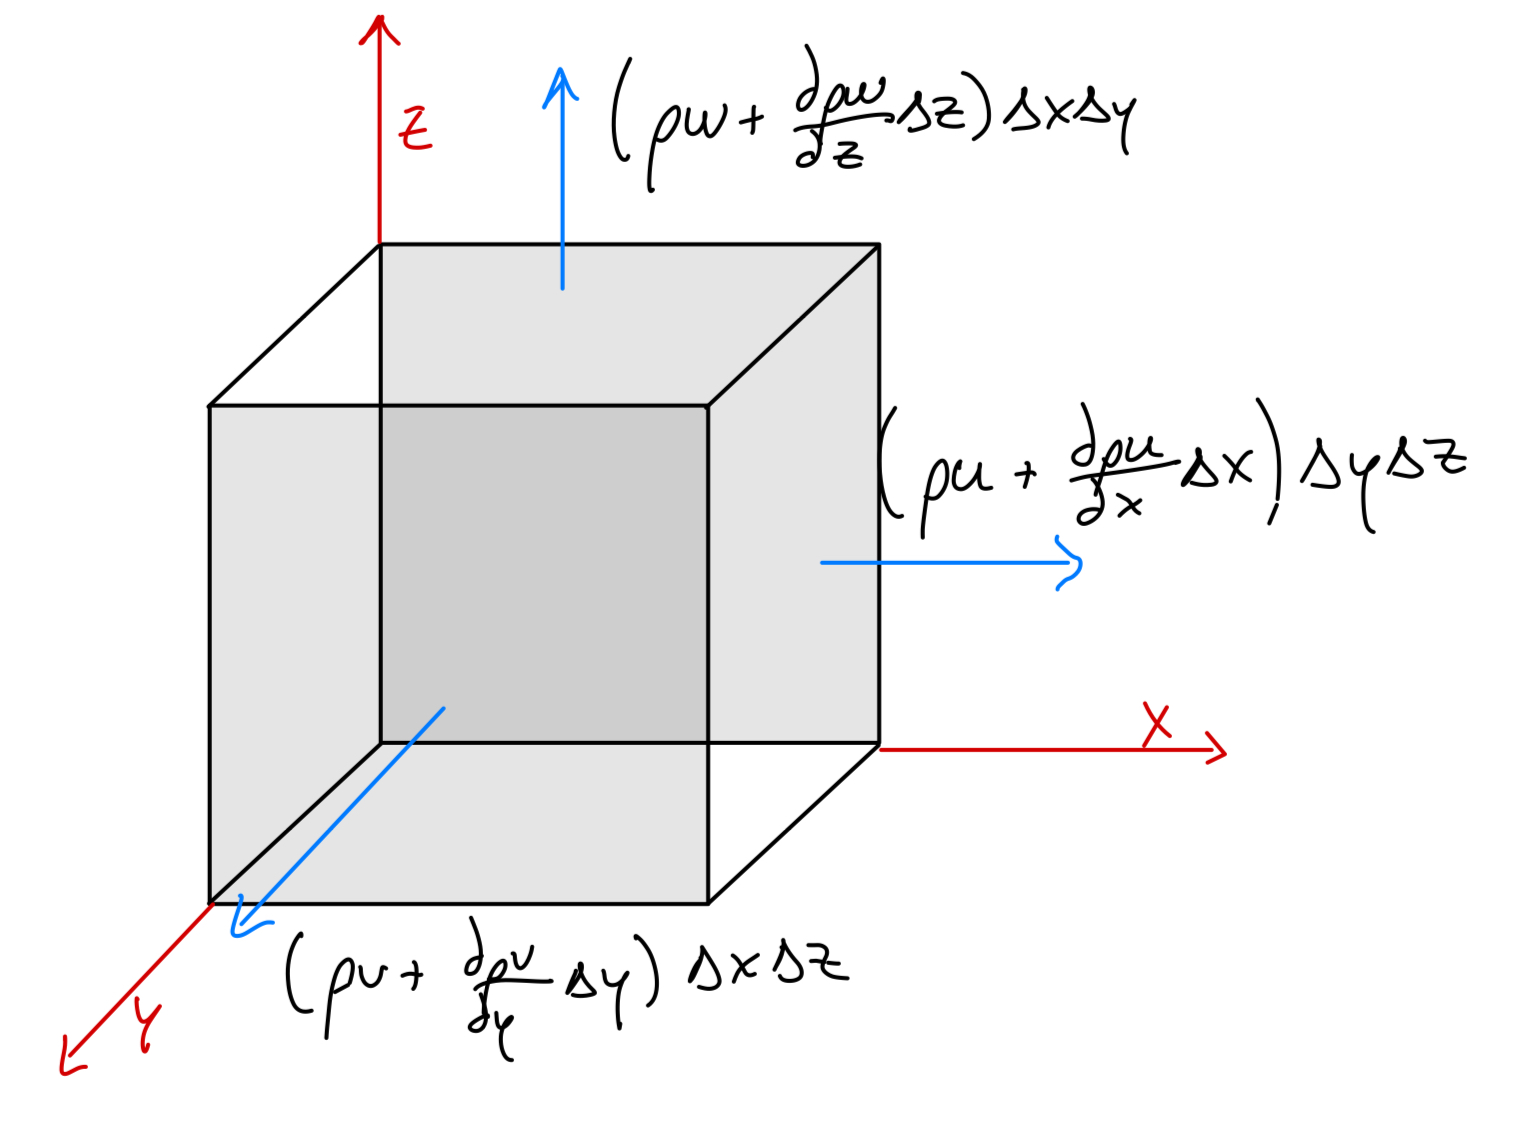
\includegraphics[width=0.5\textwidth]{FOTOS/out.jpg}
    \caption{Salida del Sistema}
    \label{fig:ley_darcy}
\end{figure}

Luego, por conservacion de masa:

\begin{equation}
    Q_{int} = Q_{out}
\end{equation}

De lo que se obtiene:

\begin{equation}
    \rho_u \Delta_y \Delta_z + \rho_v \Delta_x \Delta_z + \rho_w \Delta_x \Delta_y = (\rho_u + \frac{d\rho_u \Delta x}{dx})\Delta_y \Delta_z + (\rho_v + \frac{d\rho_v \Delta y}{dy})\Delta_x \Delta_z + (\rho_w + \frac{d\rho_w \Delta z}{dz})\Delta_x \Delta_y
\end{equation}

Simplificando:

\begin{equation}
    \Delta_x \Delta_y \Delta_z = Volumen
\end{equation}

Pero el fluido al ser agua es incompresible, por lo tanto:

\begin{equation}
   -\rho(\frac{du}{dx}+ \frac{dv}{dy}+ \frac{dw}{dz}) = 0
\end{equation}

Lo que es analogo a decir:

\begin{equation}
    -\rho \nabla \cdot \vec{v} = 0 = \nabla \cdot \vec{v}
\end{equation}

Por lo tanto, si reemplazamos en la ley de Darcy, obtenemos:

\begin{equation}
    V_x = k_x\cdot \frac{dh}{dx}; V_y = k_y\cdot \frac{dh}{dy}; V_z = k_z\cdot \frac{dh}{dz}
\end{equation}

Incroporando la ecuacion de continuidad, se obtiene:

\begin{equation}
    \nabla \cdot \vec{V} = \nabla \cdot (k \cdot \vec{i}) = 0
\end{equation}

Asumiendo un analisis en 2D, se obtiene:

\begin{equation}
    \frac{d}{dx}(k_x \cdot \frac{dh}{dx}) + \frac{d}{dy}(k_y \cdot \frac{dh}{dy}) = 0
\end{equation}

Pero sabemos, o mejor dicho, suponemos que:

\begin{equation}
    k_x = k_y = k
\end{equation}

Por lo tanto:

\begin{equation}
    k \nabla^2 h = 0
\end{equation}

De esta forma, podemos representar el laplaciano con diferencias finitas:

\subsection{Diferencias Finitas}

\subsubsection{Diferencias Hacia Delante}

\begin{equation}
    h(x + \Delta x) = h(x) + \frac{dh}{dx} \Delta x + ...
\end{equation}

\subsubsection{Diferencias Hacia Atras}

\begin{equation}
    h(x - \Delta x) = h(x) - \frac{dh}{dx} \Delta x + ...-...+
\end{equation}

\subsubsection{Diferencias Centrales}

Se representa como la suma de una diferencia hacia delante y hacia atras, obteniendo:

\begin{equation}
    h(x + \Delta x) + h(x - \Delta x) = h(x) + \frac{d^2h}{dx^2}\frac{\Delta x}{2!} + ...(los pares)
\end{equation}

Donde la incognita que se busca es $\frac{d^2h}{dx^2}$, por lo tanto, y despejando, se obtiene:

\begin{equation}
    \frac{d^2h}{dx^2} = \frac{h(x + \Delta x) - 2h(x) + h(x - \Delta x)}{\Delta x^2}
\end{equation}

\begin{equation}
    \frac{dh}{dx} = \frac{h(x + \Delta x) - h(x)}{\Delta x}
\end{equation}

Lo cual se puede llevar a una grilla:
\\ \\
PONER IMAGEN!!!
\\ \\
Donde se puede representar la ecuacion de Laplace como:

\begin{equation}
    \frac{d^2h}{dx^2} = \frac{h_{i+1,j} + h_{i-1,j} - 2h_{i,j}}{\Delta x^2}
\end{equation}

\begin{equation}
    \frac{dh}{dx} = \frac{h_{+1,j} + h_{i+1,j} }{2\Delta x}
\end{equation}

Por lo tanto, podemos expresar la ley de Darcy con diferencias centrales, obteniendo:

\begin{equation}
    \frac{k}{\Delta^2}(h_{i+1,j} + h_{i-1,j} + h_{i,j+1} + h_{i,j-1} - 4h_{i,j}) = 0
\end{equation}

Donde se busca:

\begin{equation}
    h_{i,j} = \frac{1}{4}(h_{i+1,j} + h_{i-1,j} + h_{i,j+1} + h_{i,j-1})
\end{equation}

De esta forma, es posible ir obteniendo las diferentes variaciones en el potencial, a partir de los datos conocidos en la grilla (condiciones de borde).

\newpage
\section{Desarollo}

Para expplicar el desarrollo del codigo, se utilizara el caso ejemplo 1 como ejemplo, utilizando una grilla de 10x10. En primer lugar, se desarrolla la matriz de potencial con las condiciones de borde:

\begin{center}
    \begin{tabular}{|c|c|c|c|c|c|c|c|c|c|} 
        \hline
        \textbf{0} & \textbf{300} & \textbf{300} & \textbf{300} & \textbf{300} & \textbf{0} & \textbf{380} & \textbf{380} & \textbf{380} & \textbf{0} \\
        \hline
        \textbf{0} & \textbf{300} & \textbf{300} & \textbf{300} & \textbf{300} & \textbf{0} & 1 & 1 & 1 & \textbf{0} \\
        \hline
        \textbf{0} & \textbf{300} & \textbf{300} & \textbf{300} & \textbf{300} & \textbf{0} & 1 & 1 & 1 & \textbf{0} \\
        \hline
        \textbf{0} & \textbf{300} & \textbf{300} & \textbf{300} & \textbf{300} & \textbf{0} & 1 & 1 & 1 & \textbf{0} \\
        \hline
        \textbf{0} & 1 & 1 & 1 & 1 & 1 & 1 & 1 & 1 & \textbf{0} \\
        \hline
        \textbf{0} & 1 & 1 & 1 & 1 & 1 & 1 & 1 & 1 & \textbf{0} \\
        \hline
        \textbf{0} & 1 & 1 & 1 & 1 & 1 & 1 & 1 & 1 & \textbf{0} \\
        \hline
        \textbf{0} & 1 & 1 & 1 & 1 & 1 & 1 & 1 & 1 & \textbf{0} \\
        \hline
        \textbf{0} & 1 & 1 & 1 & 1 & 1 & 1 & 1 & 1 & \textbf{0} \\
        \hline
        \textbf{0} & \textbf{0} & \textbf{0} & \textbf{0} & \textbf{0} & \textbf{0} & \textbf{0} & \textbf{0} & \textbf{0} & \textbf{0} \\
        \hline
    \end{tabular}
\end{center}

Donde se observan las condiciones de impermeabilidad expuestas \textbf{(0)}, la condicion de inicio de flujo \textbf{(380)} y la condicion de flujo final \textbf{(300)}, donde, por razones de logica de codigo, se rellena con esta valor en los espacios con aire. Luego, iterando segun la teoria expuesta anteriormente, y manteniendo las condiciones de borde se obtiene lo siguiente:

\begin{center}
    \begin{tabular}{|c|c|c|c|c|c|c|c|c|c|} 
        \hline
        \textbf{0} & \textbf{300} & \textbf{300} & \textbf{300} & \textbf{300} & \textbf{0} & \textbf{380} & \textbf{380} & \textbf{380} & \textbf{0} \\
        \hline
        \textbf{0} & \textbf{300} & \textbf{300} & \textbf{300} & \textbf{300} & \textbf{0} & 365 & 366 & 367 & \textbf{0} \\
        \hline
        \textbf{0} & \textbf{300} & \textbf{300} & \textbf{300} & \textbf{300} & \textbf{0} & 351 & 353 & 354 & \textbf{0} \\
        \hline
        \textbf{0} & \textbf{300} & \textbf{300} & \textbf{300} & \textbf{300} & 317 & 334 & 341 & 343 & \textbf{0} \\
        \hline
        \textbf{0} & 303 & 304 & 305 & 309 & 317 & 327 & 332 & 335 & \textbf{0} \\
        \hline
        \textbf{0} & 306 & 307 & 309 & 312 & 318 & 323 & 327 & 329 & \textbf{0} \\
        \hline
        \textbf{0} & 309 & 310 & 311 & 314 & 318 & 321 & 324 & 326 & \textbf{0} \\
        \hline
        \textbf{0} & 310 & 311 & 313 & 315 & 318 & 320 & 322 & 324 & \textbf{0} \\
        \hline
        \textbf{0} & 311 & 312 & 313 & 315 & 318 & 320 & 322 & 323 & \textbf{0} \\
        \hline
        \textbf{0} & \textbf{0} & \textbf{0} & \textbf{0} & \textbf{0} & \textbf{0} & \textbf{0} & \textbf{0} & \textbf{0} & \textbf{0} \\
        \hline
    \end{tabular}         
\end{center}

Este es un proceso iterativo, donde se determina que la condicion de finalizacion corresponde a un error de \textbf{1e-6}.
\\ \\
Posteriormente, es posible obtener las matrices de valocidades de la siguiente manera:

\begin{lstlisting}[language=Python]
    # Calcular el gradiente del potencial (flujo de velocidad)
    dy, dx = np.gradient(potential, dy, dx)

    #Luego, el gradiente se multiplica por la permeabilidad K
    velocity_x = -dx * K 
    velocity_y = -dy * K
\end{lstlisting}

A continuacion se presentaran los distintos resultados obtenidos, donde se utilizo una grilla de 60x60 en cada caso.

\subsection{Caso 1}

\begin{figure}[H]
    \centering
    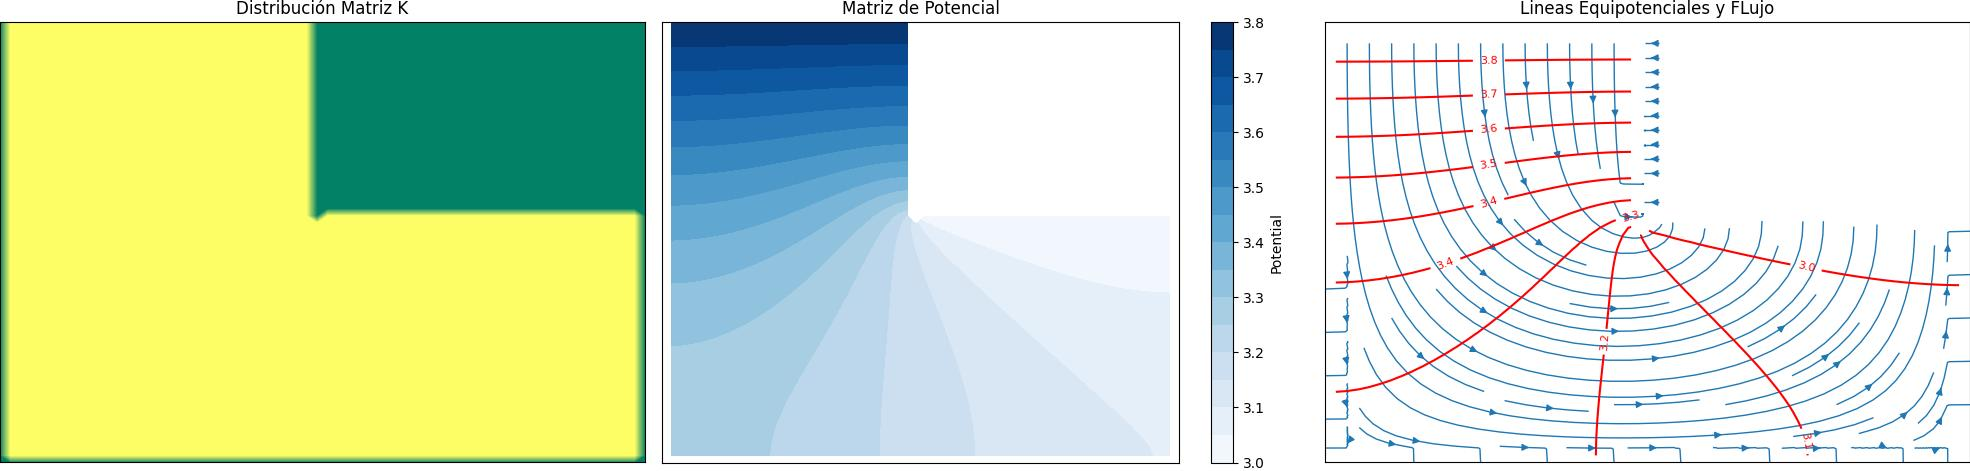
\includegraphics[width=1\textwidth]{GRAFICOS/laplace_caso_1.jpg}
    \caption{Gráfico de la función $f(x) = x^2$}
    \label{fig:caso_1}
\end{figure}

Se alcanzo la convergencia en la \textbf{iteracion 10588}
\\ \\
La velocidad de salida obtenida fue de \textbf{2.44e-05} m/s

\subsection{Caso 2}

\begin{figure}[H]
    \centering
    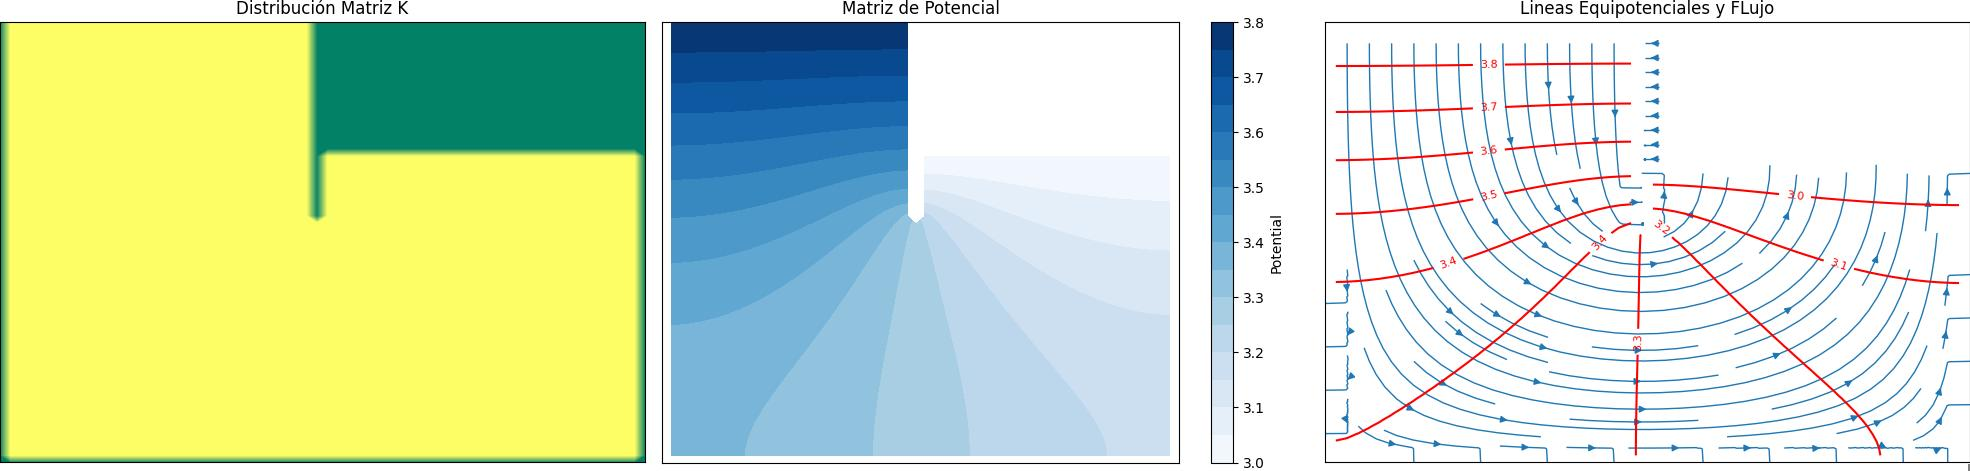
\includegraphics[width=1\textwidth]{GRAFICOS/laplace_caso_2.jpg}
    \caption{Gráfico de la función $f(x) = x^2$}
    \label{fig:caso_2}
\end{figure}

Se alcanzo la convergencia en la \textbf{iteracion 15651}
\\ \\
La velocidad de salida obtenida fue de \textbf{2.71e-05} m/s

\subsection{Caso 3}

\begin{figure}[H]
    \centering
    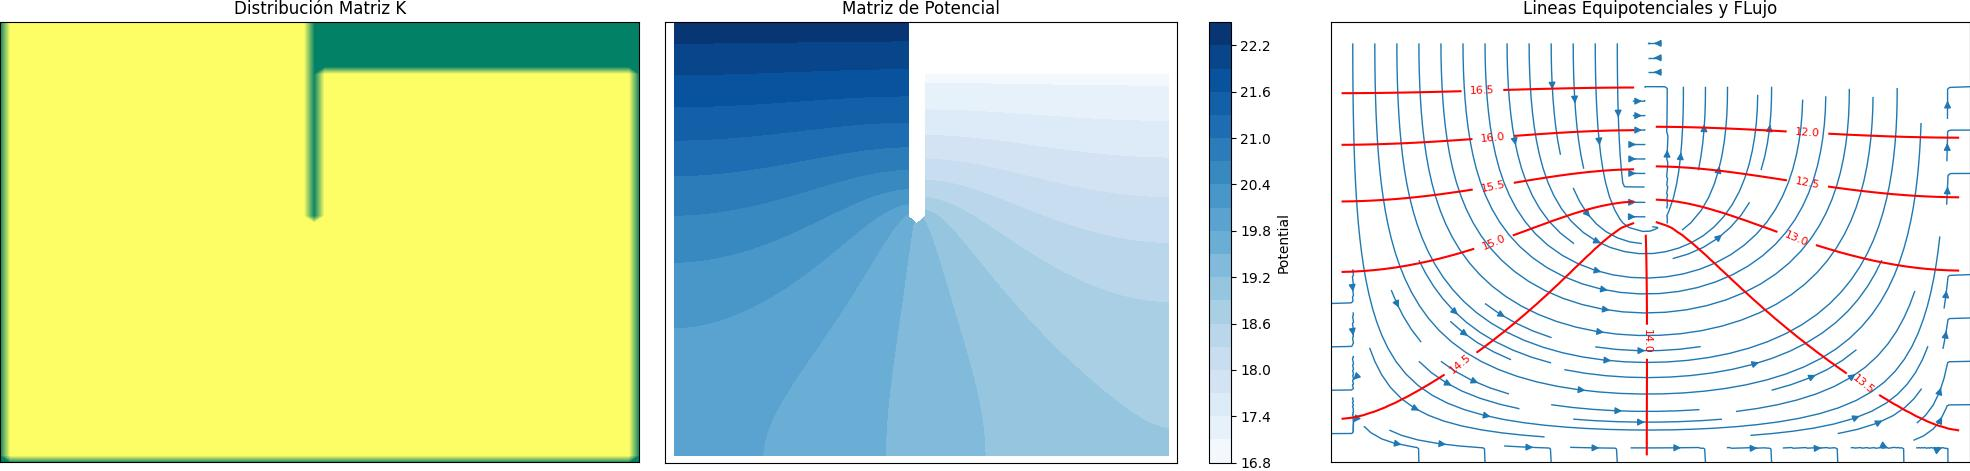
\includegraphics[width=1\textwidth]{GRAFICOS/laplace_caso_3.jpg}
    \caption{Gráfico de la función $f(x) = x^2$}
    \label{fig:caso_3}
\end{figure}

Se alcanzo la convergencia en la \textbf{iteracion 24670}
\\ \\
La velocidad de salida obtenida fue de \textbf{8.01e-05} m/s

\subsection{Caso Ejemplo Libro}

\begin{figure}[H]
    \centering
    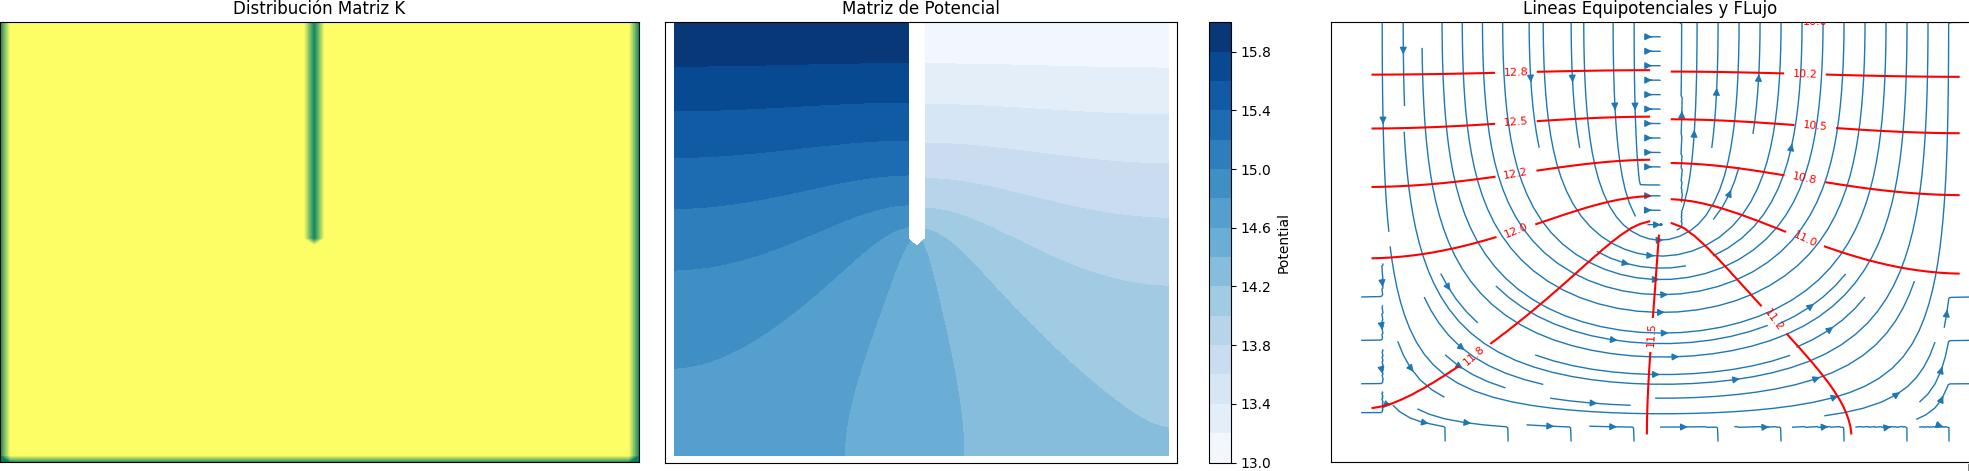
\includegraphics[width=1\textwidth]{GRAFICOS/laplace_caso_ejemplo.jpg}
    \caption{Gráfico de la función $f(x) = x^2$}
    \label{fig:caso_ejemplo}
\end{figure}

Se alcanzo la convergencia en la \textbf{iteracion 28172}
\\ \\
La velocidad de salida obtenida fue de \textbf{3.25e-06} m/s, de esta manera se corrobora que el codigo esta correctamente calibrado, ya que el resultado expuesto por el libro es de \textbf{3.2e-06} m/s.
\\ \\
Ademas, se realiza un caso doble, para ver como afecta la condicion de impermeabilidad de la barrera derecha en el flujo:

\begin{figure}[H]
    \centering
    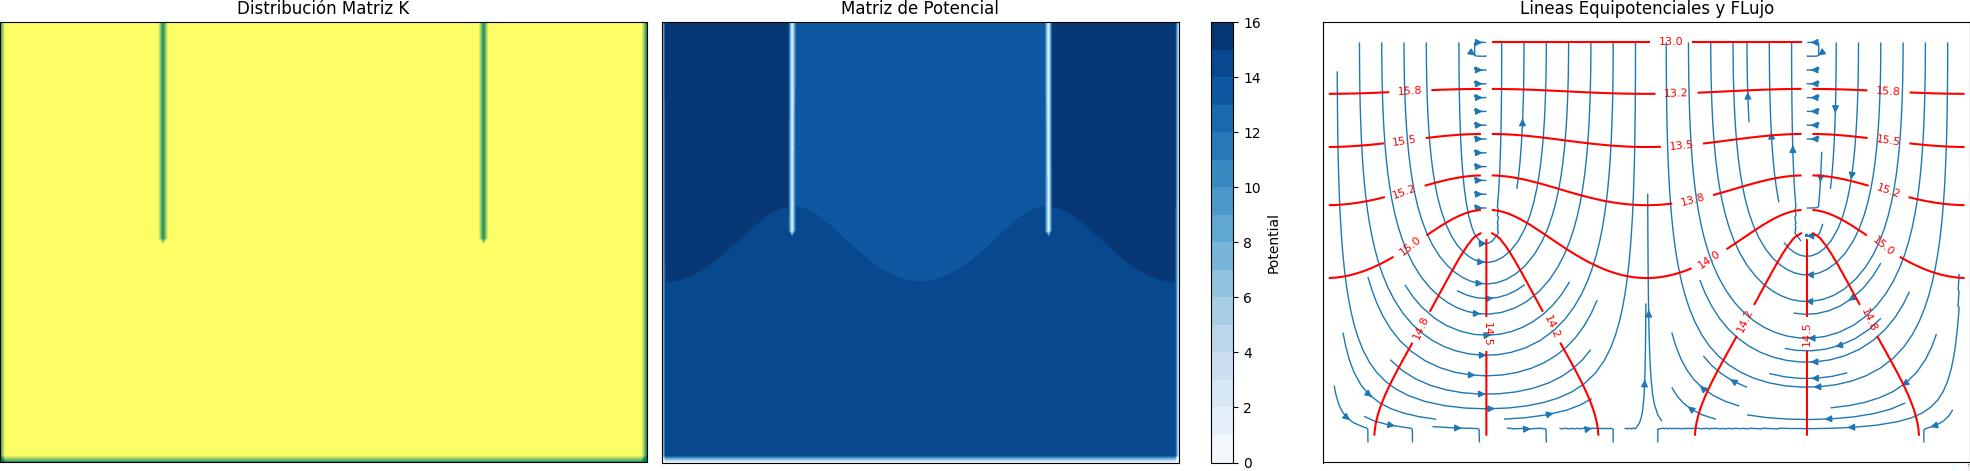
\includegraphics[width=1\textwidth]{GRAFICOS/laplace_caso_ejemplo_doble.jpg}
    \caption{Gráfico de la función $f(x) = x^2$}
    \label{fig:caso_ejemplo}
\end{figure}

Se alcanzo la convergencia en la \textbf{iteracion 16708}
\\ \\
La velocidad de salida obtenida fue de \textbf{2.63e-06} m/s.